
\documentclass[10pt,a4paper]{article}
\usepackage[utf8]{inputenc}
\usepackage[french]{babel}
\usepackage[left=2cm,right=2cm,top=2cm,bottom=2cm]{geometry}
\usepackage{hyperref}
\usepackage{graphicx}

%opening
\title{COLD2 – TP 01 – Hadoop, Spark, Kafka et HBase}
\author{Nicolas Vadkerti}
\usepackage{listings} % Required for inserting code snippets
\usepackage[usenames,dvipsnames]{color} % Required for specifying custom colors and referring to colors by name

\definecolor{DarkGreen}{rgb}{0.0,0.4,0.0} % Comment color
\definecolor{highlight}{RGB}{255,251,204} % Code highlight color

\lstdefinestyle{Style1}{ % Define a style for your code snippet, multiple definitions can be made if, for example, you wish to insert multiple code snippets using different programming languages into one document
language=Perl, % Detects keywords, comments, strings, functions, etc for the language specified
backgroundcolor=\color{highlight}, % Set the background color for the snippet - useful for highlighting
basicstyle=\footnotesize\ttfamily, % The default font size and style of the code
breakatwhitespace=false, % If true, only allows line breaks at white space
breaklines=true, % Automatic line breaking (prevents code from protruding outside the box)
captionpos=b, % Sets the caption position: b for bottom; t for top
commentstyle=\usefont{T1}{pcr}{m}{sl}\color{DarkGreen}, % Style of comments within the code - dark green courier font
deletekeywords={}, % If you want to delete any keywords from the current language separate them by commas
%escapeinside={\%}, % This allows you to escape to LaTeX using the character in the bracket
firstnumber=1, % Line numbers begin at line 1
frame=single, % Frame around the code box, value can be: none, leftline, topline, bottomline, lines, single, shadowbox
frameround=tttt, % Rounds the corners of the frame for the top left, top right, bottom left and bottom right positions
keywordstyle=\color{Blue}\bf, % Functions are bold and blue
morekeywords={}, % Add any functions no included by default here separated by commas
numbers=left, % Location of line numbers, can take the values of: none, left, right
numbersep=10pt, % Distance of line numbers from the code box
numberstyle=\tiny\color{Gray}, % Style used for line numbers
rulecolor=\color{black}, % Frame border color
showstringspaces=false, % Don't put marks in string spaces
showtabs=false, % Display tabs in the code as lines
stepnumber=5, % The step distance between line numbers, i.e. how often will lines be numbered
stringstyle=\color{Purple}, % Strings are purple
tabsize=2
}

\newcommand{\insertcode}[2]{\begin{itemize}\item[]\lstinputlisting[caption=#2,label=#1,style=Style1]{#1}\end{itemize}} 


% \insertcode{"Scripts/example.pl"}{Nena would be proud.} 

\begin{document}

\maketitle


\url{https://github.com/SlaynPool/CR_COLD2/}
\section{Démarrage du cluster Hadoop}
\subsection{Récupérer l’image Hadoop sur le registre docker de l’IUT}
On utilise la version 3.2.0 car la 3.2.1 ne fonctionne pas. Cela ne gene pas pour le bon déroulement du TP.
\insertcode{commande/1.txt}{Docker Pull}

\subsection{Créer un pont réseau docker pour le cluster Hadoop}
On crée une nouvelle interface
 \insertcode{commande/2.txt}{Docker network}
\subsection{Lancer les conteneurs docker Hadoop à l’aide du script fourni} 
\insertcode{commande/3.txt}{Creation des conteneurs}
\subsection{Exécuter enfin le script de démarrage du cluster Hadoop}
\insertcode{commande/4.txt}{Démarrage du CLuster}
\subsection{Afficher   alors   la   liste   des   processus   JAVA   en   fonctionnement   sur  hadoop-master  avec   lacommande jps.}
Voici donc la liste des processus JAVA listé par JPS une commande propre a JAVA.
\insertcode{commande/5.txt}{Processus Java}
\subsection{Afficher ensuite l’état du système HDFS et noter le nom des 2 machines esclaves du cluster}
Execution de la commande:
\insertcode{commande/6.txt}{HDFS}
On peut voir que nous avons 2 noeuds de données répartis sur 2 machines. hadoop-slave1 et hadoop-slave2
\subsection{Comparer aux informations disponibles sur l’URL http://localhost:9870/}
\begin{figure}[h!]
\centering
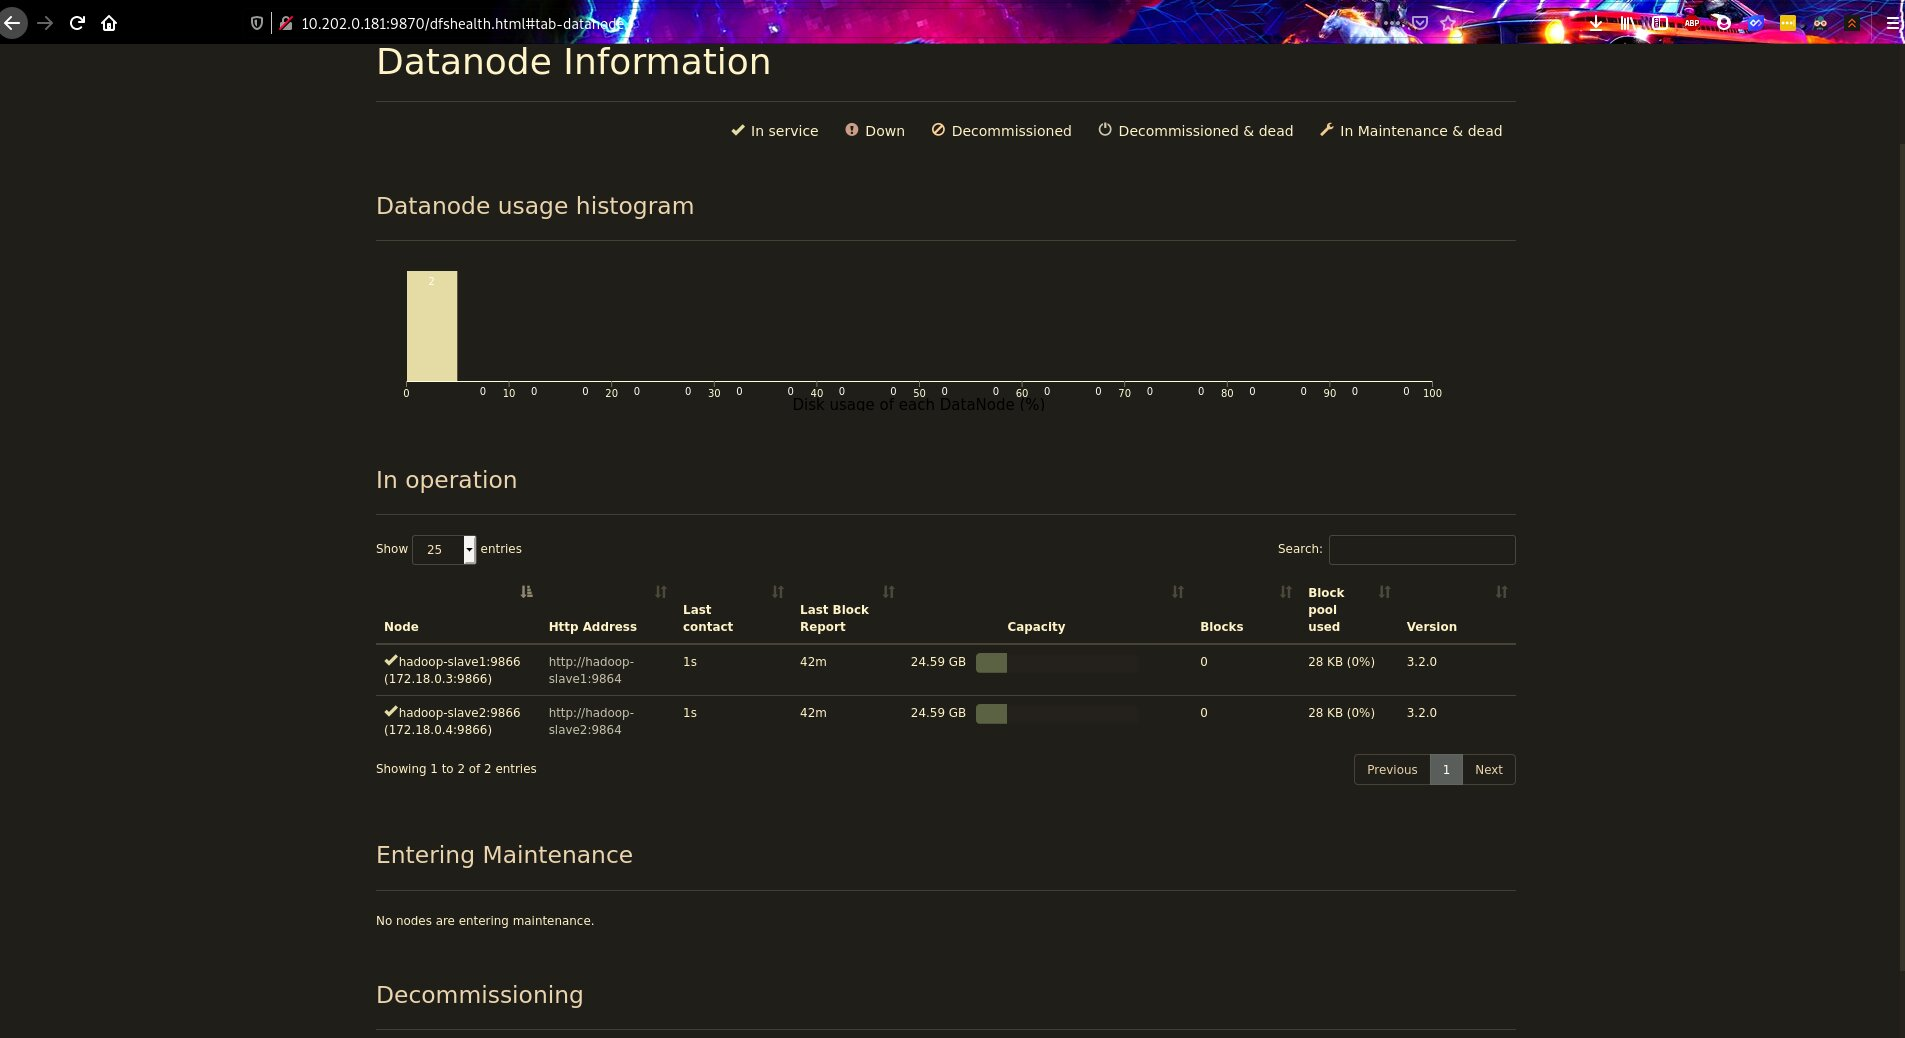
\includegraphics[scale=0.20]{image/1.jpg}
\caption{Interface Web }
\label{fig:net }
\end{figure}
On peut voir que les machines esclaves sont appellé par des noms de domaines. De plus, on voit que l'espaces est repartie de moitié sur chaques noeuds.

\subsection{Comment   modifier   la   machine   locale   pour   que   l’on   puisse   cliquer   sur   les   liens   de   la   page«Datanodes» (http://hadoop-slave1:9864 et http://hadoop-slave2:9864 ) }

PAUSE

\subsection{Créer ensuite le répertoire de base pour l’utilisateur root}
\insertcode{commande/7.txt}{Creation du FS }

\subsection{Tester alors les options -ls, -put, -get, -mv, -rm, -cat, -tail de la commande hadoop fs}
\insertcode{commande/8.txt}{Manipulation du FS }


\end{document}

